\section{Weight duplications}
One of the optimizations the compiler may perform to improve the inference latency is to use segmentation on certain layers (e.g., convolutional layers).
This segmentation allows a layer to be segmented so that it can be executed in parallel (i.e., tensor parallelism).
Performing this technique on the \graicore{}, so that a layer can be executed on multiple cores at the same time, certain weights must be present on the respective neuron cores.
In other words, this means that on the \graicore{}, there are duplicate weights present.

A naive approach to configure a model is to read every weight, including duplicate weights, from the external memory.
However, we have seen in \cref{section:energy_evaluation} that in the configuration process, reading from the LPDDR5X memory consumes the most energy.

There is an opportunity in decreasing the energy cost for reading from the external DDR memory.
Instead of reading all the weights (including duplicates), we can read only the unique duplicates once.
For this to work however, we require a separate controller (close to the \graicore{}) that can copy and distribute the weights to the neuron cores that require them.

Let's first look why this technique is interesting to pursue.
To determine the number of duplicates that are present in the compiled model, we do the following:
\begin{enumerate}
    \item
    Count the number of relevant parameters ($w_\textrm{original}$) in the original model.
    \item
    Retrieve the number of bytes required for weights for the compiled model ($d_\textrm{weights}$).
    \item
    Compute the number of weights in the compiled model by taking quantization into account ($w_\textrm{compiled} = d_\textrm{weights} \times \frac{8}{q}$ with $q$ as the quantization value (e.g., $8$, $16$ or $32$)).
    \item  
    The number of duplicate weights can then be calculated by subtracting weights from the compiled model with the parameters counted from the original model. That is, $w_\textrm{dupes} = w_\textrm{compiled} - w_\textrm{original}$.
\end{enumerate}

\begin{table}[hbtp]
\centering
\begin{tabular}{@{}lr@{}}
\toprule
\textbf{Model}          & \textbf{Weight duplication ratio} \\ \midrule
efficientnet            & 22\%                              \\
mobnetv2                & 17\%                              \\
object\_tracker         & 40\%                              \\
object\_detector        & 74\%                              \\
resnet50                & 46\%                              \\
resnet101\_p0           & 53\%                              \\
resnet101\_p1           & 51\%                              \\
resnet101\_p2           & 51\%                              \\
resnet101\_p3           & 23\%                              \\
resnet101\_p4           & 2\%                               \\
resnet101\_pruned\_p0   & 58\%                              \\
resnet101\_pruned\_p1   & 59\%                              \\
resnet101\_pruned\_p2   & 59\%                              \\
resnet101\_pruned\_p3   & 38\%                              \\
resnet101\_pruned\_p4   & 20\%                              \\ \bottomrule
\end{tabular}
\caption{Ratio of weight duplicates for each example model}
\label{tab:example_models_duplicate_weights}
\end{table}

The number of weight duplicates is dependent on the model and how the compiler performed the mapping of the original model.
\Cref{tab:example_models_duplicate_weights} shows for various models the percentage of duplicate weights.
We observe that up to 74\% of the weights are duplicates with an average of 41\%.
Since weights are in most cases the largest component of the total compiled model size, these numbers show that there is potentially notable savings in configuration performance.

Note that this technique requires additional logic to be added to the system which acts as a component that transfers copies of relevant weights to multiple destination SRAMs.
This, of course, also adds to the total energy consumption when performing a configuration.
However, such a component has not been analyzed and is not included in the preliminary energy analysis. 
We assumed that the amount of data read from the external memory is decreased by the number of duplicate weights.
Also, less data has to be transferred through the PHY, controller and AXI.
The energy consumed by the \confignoc{} and SRAMs are the same as in the scenario where we include the weights duplicates.

\Cref{fig:resnet50_weight_duplicates} shows the energy distribution of the ResNet-50, including and excluding the reading of duplicate weights. 
We observe an configuration energy decrease of 12\%.

\begin{figure}[hbtp]
    \centering
    \subcaptionbox{Includes weight duplicates}{
        \def\printonlylargeenough#1#2{{\unless\ifdim#2pt<#1pt\relax
#2\printnumbertrue
\else
\printnumberfalse
\fi}}
\newif\ifprintnumber

\begin{tikzpicture}
    \pie[
        radius=2.5,
        text=pin,
        hide number,
    ]{
        1.0/1.0\%,
        13.9/13.9\%,
        4.0/4.0\%,
        2.4/2.4\%
    }
    \pie[
        radius=2.5,
        hide number,
        color={gray, bluehue2, bluehue4, bluehue6},
        before number=\printonlylargeenough{2},
        after number=\ifprintnumber\%\fi
    ]{
        1.0/,
        13.9/,
        4.0/,
        2.4/
    }
    \pie[
        radius=2,
        text=inside,
        color={blue!60, red!60},
    ]{
        21.3/$\econf$,
        78.7/$\eproc$
    }
\end{tikzpicture}
    }
    \hfill
    \subcaptionbox*{}[0em]{
        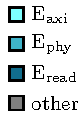
\includegraphics{assets/legend.pdf}
    }
    \hfill
    \subcaptionbox{Excludes weight duplicates}{
        \def\printonlylargeenough#1#2{{\unless\ifdim#2pt<#1pt\relax
#2\printnumbertrue
\else
\printnumberfalse
\fi}}
\newif\ifprintnumber

\begin{tikzpicture}
    \pie[
        radius=2.5,
        text=pin,
        hide number,
    ]{
        0.8/0.8\%,
        12.2/12.2\%,
        3.5/3.5\%,
        2.1/2.1\%
    }
    \pie[
        radius=2.5,
        hide number,
        color={gray, bluehue2, bluehue4, bluehue6},
        before number=\printonlylargeenough{2},
        after number=\ifprintnumber\%\fi
    ]{
        0.8/,
        12.2/,
        3.5/,
        2.1/
    }
    \pie[
        radius=2,
        text=inside,
        color={blue!60, red!60},
    ]{
        18.7/$\econf$,
        81.3/$\eproc$
    }
\end{tikzpicture}
    }
    \caption{ResNet-50 weight duplicates. Using LPDDR5X memory.}
    \label{fig:resnet50_weight_duplicates}
\end{figure}
